\documentclass[1p]{elsarticle_modified}
%\bibliographystyle{elsarticle-num}

%\usepackage[colorlinks]{hyperref}
%\usepackage{abbrmath_seonhwa} %\Abb, \Ascr, \Acal ,\Abf, \Afrak
\usepackage{amsfonts}
\usepackage{amssymb}
\usepackage{amsmath}
\usepackage{amsthm}
\usepackage{scalefnt}
\usepackage{amsbsy}
\usepackage{kotex}
\usepackage{caption}
\usepackage{subfig}
\usepackage{color}
\usepackage{graphicx}
\usepackage{xcolor} %% white, black, red, green, blue, cyan, magenta, yellow
\usepackage{float}
\usepackage{setspace}
\usepackage{hyperref}

\usepackage{tikz}
\usetikzlibrary{arrows}

\usepackage{multirow}
\usepackage{array} % fixed length table
\usepackage{hhline}

%%%%%%%%%%%%%%%%%%%%%
\makeatletter
\renewcommand*\env@matrix[1][\arraystretch]{%
	\edef\arraystretch{#1}%
	\hskip -\arraycolsep
	\let\@ifnextchar\new@ifnextchar
	\array{*\c@MaxMatrixCols c}}
\makeatother %https://tex.stackexchange.com/questions/14071/how-can-i-increase-the-line-spacing-in-a-matrix
%%%%%%%%%%%%%%%

\usepackage[normalem]{ulem}

\newcommand{\msout}[1]{\ifmmode\text{\sout{\ensuremath{#1}}}\else\sout{#1}\fi}
%SOURCE: \msout is \stkout macro in https://tex.stackexchange.com/questions/20609/strikeout-in-math-mode

\newcommand{\cancel}[1]{
	\ifmmode
	{\color{red}\msout{#1}}
	\else
	{\color{red}\sout{#1}}
	\fi
}

\newcommand{\add}[1]{
	{\color{blue}\uwave{#1}}
}

\newcommand{\replace}[2]{
	\ifmmode
	{\color{red}\msout{#1}}{\color{blue}\uwave{#2}}
	\else
	{\color{red}\sout{#1}}{\color{blue}\uwave{#2}}
	\fi
}

\newcommand{\Sol}{\mathcal{S}} %segment
\newcommand{\D}{D} %diagram
\newcommand{\A}{\mathcal{A}} %arc


%%%%%%%%%%%%%%%%%%%%%%%%%%%%%5 test

\def\sl{\operatorname{\textup{SL}}(2,\Cbb)}
\def\psl{\operatorname{\textup{PSL}}(2,\Cbb)}
\def\quan{\mkern 1mu \triangleright \mkern 1mu}

\theoremstyle{definition}
\newtheorem{thm}{Theorem}[section]
\newtheorem{prop}[thm]{Proposition}
\newtheorem{lem}[thm]{Lemma}
\newtheorem{ques}[thm]{Question}
\newtheorem{cor}[thm]{Corollary}
\newtheorem{defn}[thm]{Definition}
\newtheorem{exam}[thm]{Example}
\newtheorem{rmk}[thm]{Remark}
\newtheorem{alg}[thm]{Algorithm}

\newcommand{\I}{\sqrt{-1}}
\begin{document}

%\begin{frontmatter}
%
%\title{Boundary parabolic representations of knots up to 8 crossings}
%
%%% Group authors per affiliation:
%\author{Yunhi Cho} 
%\address{Department of Mathematics, University of Seoul, Seoul, Korea}
%\ead{yhcho@uos.ac.kr}
%
%
%\author{Seonhwa Kim} %\fnref{s_kim}}
%\address{Center for Geometry and Physics, Institute for Basic Science, Pohang, 37673, Korea}
%\ead{ryeona17@ibs.re.kr}
%
%\author{Hyuk Kim}
%\address{Department of Mathematical Sciences, Seoul National University, Seoul 08826, Korea}
%\ead{hyukkim@snu.ac.kr}
%
%\author{Seokbeom Yoon}
%\address{Department of Mathematical Sciences, Seoul National University, Seoul, 08826,  Korea}
%\ead{sbyoon15@snu.ac.kr}
%
%\begin{abstract}
%We find all boundary parabolic representation of knots up to 8 crossings.
%
%\end{abstract}
%\begin{keyword}
%    \MSC[2010] 57M25 
%\end{keyword}
%
%\end{frontmatter}

%\linenumbers
%\tableofcontents
%
\newcommand\colored[1]{\textcolor{white}{\rule[-0.35ex]{0.8em}{1.4ex}}\kern-0.8em\color{red} #1}%
%\newcommand\colored[1]{\textcolor{white}{ #1}\kern-2.17ex	\textcolor{white}{ #1}\kern-1.81ex	\textcolor{white}{ #1}\kern-2.15ex\color{red}#1	}

{\Large $\underline{12a_{0499}~(K12a_{0499})}$}

\setlength{\tabcolsep}{10pt}
\renewcommand{\arraystretch}{1.6}
\vspace{1cm}\begin{tabular}{m{100pt}>{\centering\arraybackslash}m{274pt}}
\multirow{5}{120pt}{
	\centering
	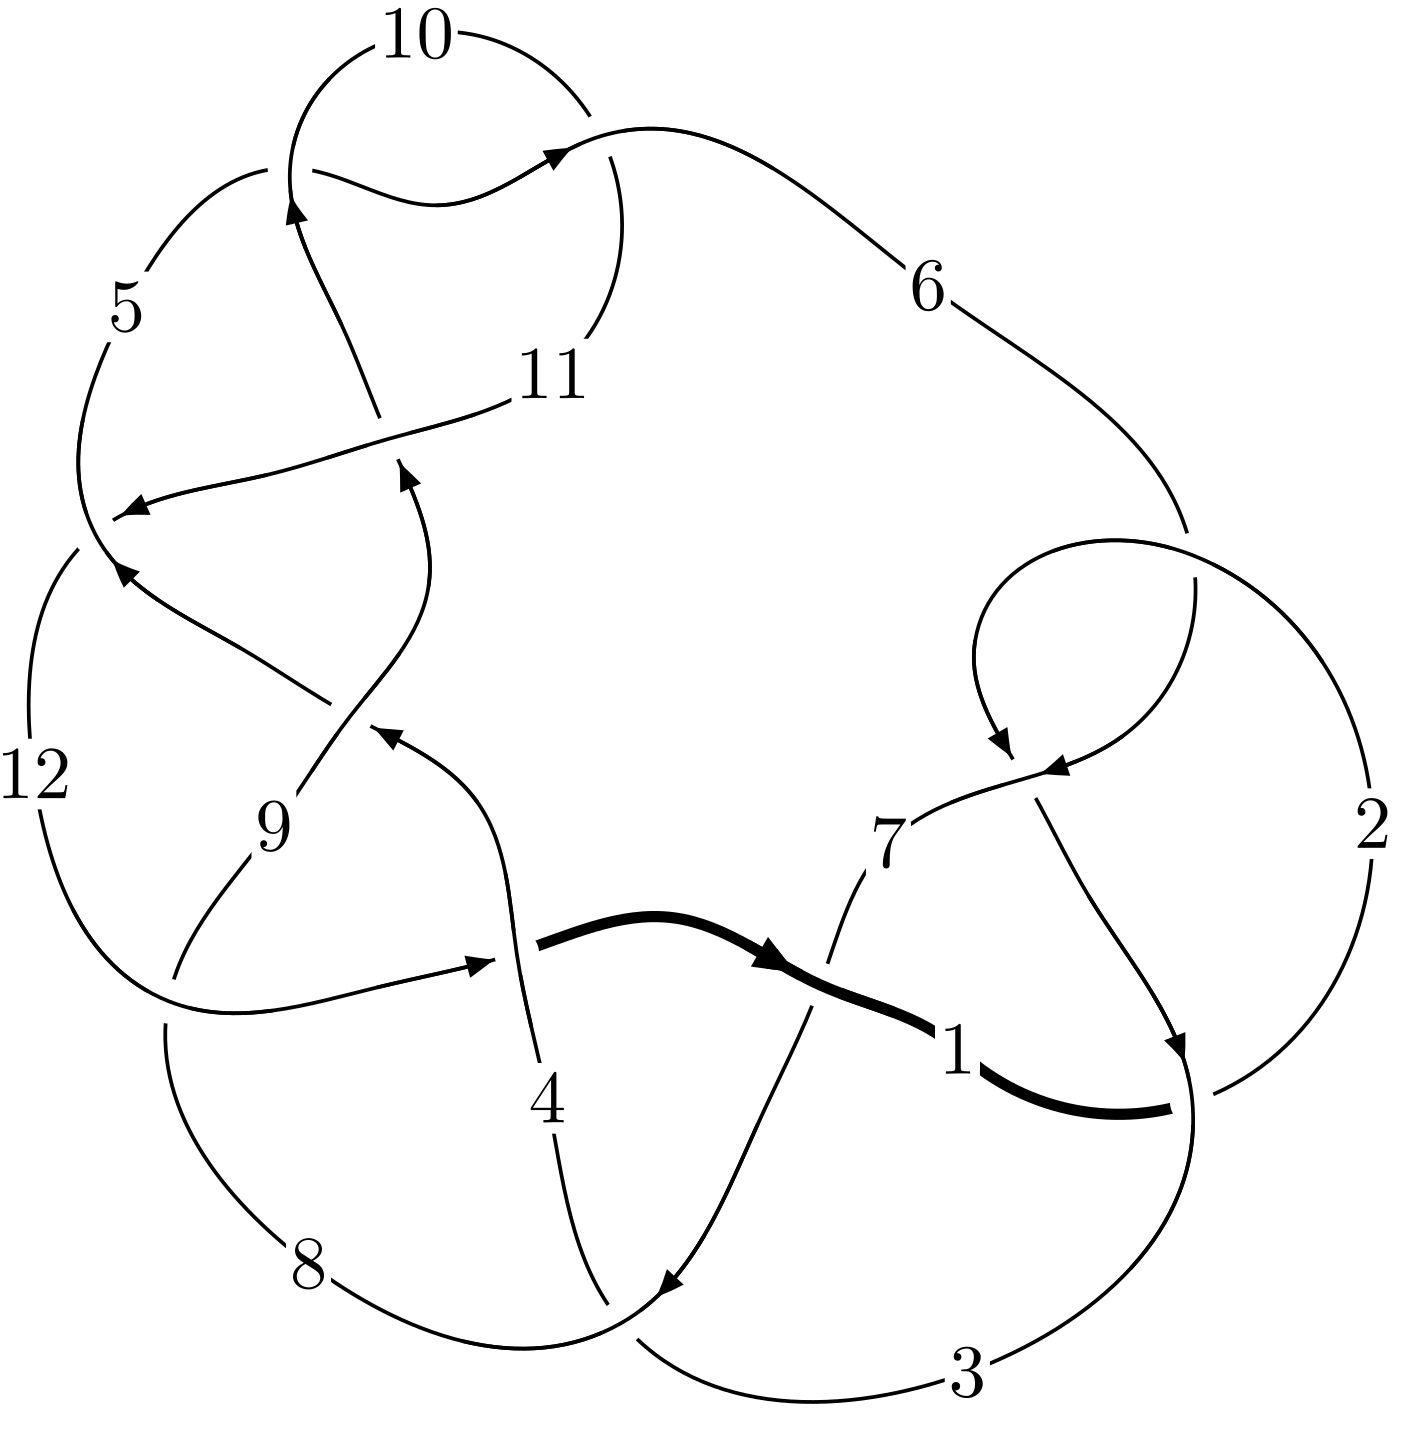
\includegraphics[width=112pt]{../../../GIT/diagram.site/Diagrams/png/1300_12a_0499.png}\\
\ \ \ A knot diagram\footnotemark}&
\allowdisplaybreaks
\textbf{Linearized knot diagam} \\
\cline{2-2}
 &
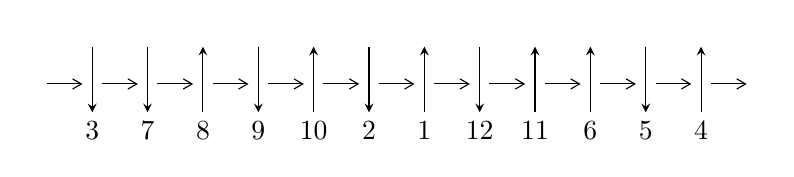
\begin{tikzpicture}[x=20pt, y=17pt]
	% nodes
	\node (C0) at (0, 0) {};
	\node (C1) at (1, 0) {};
	\node (C1U) at (1, +1) {};
	\node (C1D) at (1, -1) {3};

	\node (C2) at (2, 0) {};
	\node (C2U) at (2, +1) {};
	\node (C2D) at (2, -1) {7};

	\node (C3) at (3, 0) {};
	\node (C3U) at (3, +1) {};
	\node (C3D) at (3, -1) {8};

	\node (C4) at (4, 0) {};
	\node (C4U) at (4, +1) {};
	\node (C4D) at (4, -1) {9};

	\node (C5) at (5, 0) {};
	\node (C5U) at (5, +1) {};
	\node (C5D) at (5, -1) {10};

	\node (C6) at (6, 0) {};
	\node (C6U) at (6, +1) {};
	\node (C6D) at (6, -1) {2};

	\node (C7) at (7, 0) {};
	\node (C7U) at (7, +1) {};
	\node (C7D) at (7, -1) {1};

	\node (C8) at (8, 0) {};
	\node (C8U) at (8, +1) {};
	\node (C8D) at (8, -1) {12};

	\node (C9) at (9, 0) {};
	\node (C9U) at (9, +1) {};
	\node (C9D) at (9, -1) {11};

	\node (C10) at (10, 0) {};
	\node (C10U) at (10, +1) {};
	\node (C10D) at (10, -1) {6};

	\node (C11) at (11, 0) {};
	\node (C11U) at (11, +1) {};
	\node (C11D) at (11, -1) {5};

	\node (C12) at (12, 0) {};
	\node (C12U) at (12, +1) {};
	\node (C12D) at (12, -1) {4};
	\node (C13) at (13, 0) {};

	% arrows
	\draw[->,>={angle 60}]
	(C0) edge (C1) (C1) edge (C2) (C2) edge (C3) (C3) edge (C4) (C4) edge (C5) (C5) edge (C6) (C6) edge (C7) (C7) edge (C8) (C8) edge (C9) (C9) edge (C10) (C10) edge (C11) (C11) edge (C12) (C12) edge (C13) ;	\draw[->,>=stealth]
	(C1U) edge (C1D) (C2U) edge (C2D) (C3D) edge (C3U) (C4U) edge (C4D) (C5D) edge (C5U) (C6U) edge (C6D) (C7D) edge (C7U) (C8U) edge (C8D) (C9D) edge (C9U) (C10D) edge (C10U) (C11U) edge (C11D) (C12D) edge (C12U) ;
	\end{tikzpicture} \\
\hhline{~~} \\& 
\textbf{Solving Sequence} \\ \cline{2-2} 
 &
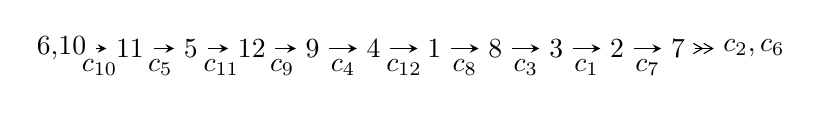
\begin{tikzpicture}[x=22pt, y=7pt]
	% node
	\node (A0) at (-1/8, 0) {6,10};
	\node (A1) at (1, 0) {11};
	\node (A2) at (2, 0) {5};
	\node (A3) at (3, 0) {12};
	\node (A4) at (4, 0) {9};
	\node (A5) at (5, 0) {4};
	\node (A6) at (6, 0) {1};
	\node (A7) at (7, 0) {8};
	\node (A8) at (8, 0) {3};
	\node (A9) at (9, 0) {2};
	\node (A10) at (10, 0) {7};
	\node (C1) at (1/2, -1) {$c_{10}$};
	\node (C2) at (3/2, -1) {$c_{5}$};
	\node (C3) at (5/2, -1) {$c_{11}$};
	\node (C4) at (7/2, -1) {$c_{9}$};
	\node (C5) at (9/2, -1) {$c_{4}$};
	\node (C6) at (11/2, -1) {$c_{12}$};
	\node (C7) at (13/2, -1) {$c_{8}$};
	\node (C8) at (15/2, -1) {$c_{3}$};
	\node (C9) at (17/2, -1) {$c_{1}$};
	\node (C10) at (19/2, -1) {$c_{7}$};
	\node (A11) at (45/4, 0) {$c_{2},c_{6}$};

	% edge
	\draw[->,>=stealth]	
	(A0) edge (A1) (A1) edge (A2) (A2) edge (A3) (A3) edge (A4) (A4) edge (A5) (A5) edge (A6) (A6) edge (A7) (A7) edge (A8) (A8) edge (A9) (A9) edge (A10) ;
	\draw[->>,>={angle 60}]	
	(A10) edge (A11);
\end{tikzpicture} \\ 

\end{tabular} \\

\footnotetext{
The image of knot diagram is generated by the software ``\textbf{Draw programme}" developed by Andrew Bartholomew(\url{http://www.layer8.co.uk/maths/draw/index.htm\#Running-draw}), where we modified some parts for our purpose(\url{https://github.com/CATsTAILs/LinksPainter}).
}\phantom \\ \newline 
\centering \textbf{Ideals for irreducible components\footnotemark of $X_{\text{par}}$} 
 
\begin{align*}
I^u_{1}&=\langle 
u^{116}+u^{115}+\cdots+2 u+1\rangle \\
\\
\end{align*}
\raggedright * 1 irreducible components of $\dim_{\mathbb{C}}=0$, with total 116 representations.\\
\footnotetext{All coefficients of polynomials are rational numbers. But the coefficients are sometimes approximated in decimal forms when there is not enough margin.}
\newpage
\renewcommand{\arraystretch}{1}
\centering \section*{I. $I^u_{1}= \langle u^{116}+u^{115}+\cdots+2 u+1 \rangle$}
\flushleft \textbf{(i) Arc colorings}\\
\begin{tabular}{m{7pt} m{180pt} m{7pt} m{180pt} }
\flushright $a_{6}=$&$\begin{pmatrix}0\\u\end{pmatrix}$ \\
\flushright $a_{10}=$&$\begin{pmatrix}1\\0\end{pmatrix}$ \\
\flushright $a_{11}=$&$\begin{pmatrix}1\\- u^2\end{pmatrix}$ \\
\flushright $a_{5}=$&$\begin{pmatrix}- u\\u\end{pmatrix}$ \\
\flushright $a_{12}=$&$\begin{pmatrix}u^4- u^2+1\\- u^4\end{pmatrix}$ \\
\flushright $a_{9}=$&$\begin{pmatrix}- u^2+1\\u^4\end{pmatrix}$ \\
\flushright $a_{4}=$&$\begin{pmatrix}- u^7+2 u^5-2 u^3\\u^9- u^7+u^5+u\end{pmatrix}$ \\
\flushright $a_{1}=$&$\begin{pmatrix}u^{20}-5 u^{18}+13 u^{16}-20 u^{14}+20 u^{12}-13 u^{10}+7 u^8-4 u^6+3 u^4- u^2+1\\- u^{22}+4 u^{20}-9 u^{18}+12 u^{16}-12 u^{14}+10 u^{12}-9 u^{10}+6 u^8-3 u^6- u^2\end{pmatrix}$ \\
\flushright $a_{8}=$&$\begin{pmatrix}u^{12}-3 u^{10}+5 u^8-4 u^6+2 u^4- u^2+1\\- u^{12}+2 u^{10}-2 u^8+u^4\end{pmatrix}$ \\
\flushright $a_{3}=$&$\begin{pmatrix}- u^{33}+8 u^{31}+\cdots-4 u^5- u\\u^{33}-7 u^{31}+\cdots+2 u^{13}+u\end{pmatrix}$ \\
\flushright $a_{2}=$&$\begin{pmatrix}u^{88}-21 u^{86}+\cdots-2 u^2+1\\- u^{88}+20 u^{86}+\cdots-5 u^8-2 u^4\end{pmatrix}$ \\
\flushright $a_{7}=$&$\begin{pmatrix}- u^{54}+13 u^{52}+\cdots-2 u^2+1\\u^{56}-12 u^{54}+\cdots+5 u^8+2 u^4\end{pmatrix}$\\&\end{tabular}
\flushleft \textbf{(ii) Obstruction class $= -1$}\\~\\
\flushleft \textbf{(iii) Cusp Shapes $= -4 u^{114}+108 u^{112}+\cdots+4 u-6$}\\~\\
\newpage\renewcommand{\arraystretch}{1}
\flushleft \textbf{(iv) u-Polynomials at the component}\newline \\
\begin{tabular}{m{50pt}|m{274pt}}
Crossings & \hspace{64pt}u-Polynomials at each crossing \\
\hline $$\begin{aligned}c_{1}\end{aligned}$$&$\begin{aligned}
&u^{116}+55 u^{115}+\cdots+2 u+1
\end{aligned}$\\
\hline $$\begin{aligned}c_{2},c_{6}\end{aligned}$$&$\begin{aligned}
&u^{116}- u^{115}+\cdots-2 u+1
\end{aligned}$\\
\hline $$\begin{aligned}c_{3}\end{aligned}$$&$\begin{aligned}
&u^{116}+u^{115}+\cdots-4460 u+481
\end{aligned}$\\
\hline $$\begin{aligned}c_{4}\end{aligned}$$&$\begin{aligned}
&u^{116}- u^{115}+\cdots+4460 u+481
\end{aligned}$\\
\hline $$\begin{aligned}c_{5},c_{10}\end{aligned}$$&$\begin{aligned}
&u^{116}+u^{115}+\cdots+2 u+1
\end{aligned}$\\
\hline $$\begin{aligned}c_{7}\end{aligned}$$&$\begin{aligned}
&u^{116}-3 u^{115}+\cdots-3102 u+1491
\end{aligned}$\\
\hline $$\begin{aligned}c_{8}\end{aligned}$$&$\begin{aligned}
&u^{116}-13 u^{115}+\cdots-28714 u+1493
\end{aligned}$\\
\hline $$\begin{aligned}c_{9}\end{aligned}$$&$\begin{aligned}
&u^{116}-55 u^{115}+\cdots-2 u+1
\end{aligned}$\\
\hline $$\begin{aligned}c_{11}\end{aligned}$$&$\begin{aligned}
&u^{116}+3 u^{115}+\cdots+3102 u+1491
\end{aligned}$\\
\hline $$\begin{aligned}c_{12}\end{aligned}$$&$\begin{aligned}
&u^{116}+13 u^{115}+\cdots+28714 u+1493
\end{aligned}$\\
\hline
\end{tabular}\\~\\
\newpage\renewcommand{\arraystretch}{1}
\flushleft \textbf{(v) Riley Polynomials at the component}\newline \\
\begin{tabular}{m{50pt}|m{274pt}}
Crossings & \hspace{64pt}Riley Polynomials at each crossing \\
\hline $$\begin{aligned}c_{1},c_{9}\end{aligned}$$&$\begin{aligned}
&y^{116}+13 y^{115}+\cdots+10 y+1
\end{aligned}$\\
\hline $$\begin{aligned}c_{2},c_{5},c_{6}\\c_{10}\end{aligned}$$&$\begin{aligned}
&y^{116}-55 y^{115}+\cdots-2 y+1
\end{aligned}$\\
\hline $$\begin{aligned}c_{3},c_{4}\end{aligned}$$&$\begin{aligned}
&y^{116}-23 y^{115}+\cdots-20059950 y+231361
\end{aligned}$\\
\hline $$\begin{aligned}c_{7},c_{11}\end{aligned}$$&$\begin{aligned}
&y^{116}+29 y^{115}+\cdots+95901630 y+2223081
\end{aligned}$\\
\hline $$\begin{aligned}c_{8},c_{12}\end{aligned}$$&$\begin{aligned}
&y^{116}+25 y^{115}+\cdots+93441422 y+2229049
\end{aligned}$\\
\hline
\end{tabular}\\~\\
\newpage\flushleft \textbf{(vi) Complex Volumes and Cusp Shapes}
$$\begin{array}{c|c|c}  
\text{Solutions to }I^u_{1}& \I (\text{vol} + \sqrt{-1}CS) & \text{Cusp shape}\\
 \hline 
\begin{aligned}
u &= -0.980916 + 0.187806 I\end{aligned}
 & -0.46811 - 4.80626 I & \phantom{-0.000000 } 0 \\ \hline\begin{aligned}
u &= -0.980916 - 0.187806 I\end{aligned}
 & -0.46811 + 4.80626 I & \phantom{-0.000000 } 0 \\ \hline\begin{aligned}
u &= \phantom{-}1.038040 + 0.264208 I\end{aligned}
 & \phantom{-}1.92758 + 0.70552 I & \phantom{-0.000000 } 0 \\ \hline\begin{aligned}
u &= \phantom{-}1.038040 - 0.264208 I\end{aligned}
 & \phantom{-}1.92758 - 0.70552 I & \phantom{-0.000000 } 0 \\ \hline\begin{aligned}
u &= \phantom{-}0.946091 + 0.512909 I\end{aligned}
 & \phantom{-}0.924676 + 0.744595 I & \phantom{-0.000000 } 0 \\ \hline\begin{aligned}
u &= \phantom{-}0.946091 - 0.512909 I\end{aligned}
 & \phantom{-}0.924676 - 0.744595 I & \phantom{-0.000000 } 0 \\ \hline\begin{aligned}
u &= -1.060920 + 0.213508 I\end{aligned}
 & -1.38450 + 2.53956 I & \phantom{-0.000000 } 0 \\ \hline\begin{aligned}
u &= -1.060920 - 0.213508 I\end{aligned}
 & -1.38450 - 2.53956 I & \phantom{-0.000000 } 0 \\ \hline\begin{aligned}
u &= -0.814804 + 0.409673 I\end{aligned}
 & -0.25942 - 4.77611 I & \phantom{-0.000000 } 0 \\ \hline\begin{aligned}
u &= -0.814804 - 0.409673 I\end{aligned}
 & -0.25942 + 4.77611 I & \phantom{-0.000000 } 0 \\ \hline\begin{aligned}
u &= -0.628886 + 0.653348 I\end{aligned}
 & -3.77819 - 10.54700 I & \phantom{-0.000000 } 0 \\ \hline\begin{aligned}
u &= -0.628886 - 0.653348 I\end{aligned}
 & -3.77819 + 10.54700 I & \phantom{-0.000000 } 0 \\ \hline\begin{aligned}
u &= \phantom{-}0.942453 + 0.559925 I\end{aligned}
 & -0.504439 - 0.872368 I & \phantom{-0.000000 } 0 \\ \hline\begin{aligned}
u &= \phantom{-}0.942453 - 0.559925 I\end{aligned}
 & -0.504439 + 0.872368 I & \phantom{-0.000000 } 0 \\ \hline\begin{aligned}
u &= -0.940053 + 0.570126 I\end{aligned}
 & -2.86201 + 5.76865 I & \phantom{-0.000000 } 0 \\ \hline\begin{aligned}
u &= -0.940053 - 0.570126 I\end{aligned}
 & -2.86201 - 5.76865 I & \phantom{-0.000000 } 0 \\ \hline\begin{aligned}
u &= \phantom{-}0.625796 + 0.644391 I\end{aligned}
 & -1.43505 + 5.59418 I & \phantom{-0.000000 } 0 \\ \hline\begin{aligned}
u &= \phantom{-}0.625796 - 0.644391 I\end{aligned}
 & -1.43505 - 5.59418 I & \phantom{-0.000000 } 0 \\ \hline\begin{aligned}
u &= -0.608287 + 0.651469 I\end{aligned}
 & -5.84997 - 2.81500 I & \phantom{-0.000000 } 0 \\ \hline\begin{aligned}
u &= -0.608287 - 0.651469 I\end{aligned}
 & -5.84997 + 2.81500 I & \phantom{-0.000000 } 0 \\ \hline\begin{aligned}
u &= -0.960180 + 0.566648 I\end{aligned}
 & -4.81422 - 1.94454 I & \phantom{-0.000000 } 0 \\ \hline\begin{aligned}
u &= -0.960180 - 0.566648 I\end{aligned}
 & -4.81422 + 1.94454 I & \phantom{-0.000000 } 0 \\ \hline\begin{aligned}
u &= \phantom{-}0.625750 + 0.608379 I\end{aligned}
 & \phantom{-0.000000 -}3.73398 I & \phantom{-0.000000 } 0. - 6.64937 I \\ \hline\begin{aligned}
u &= \phantom{-}0.625750 - 0.608379 I\end{aligned}
 & \phantom{-0.000000 } -3.73398 I & \phantom{-0.000000 -}0. + 6.64937 I \\ \hline\begin{aligned}
u &= \phantom{-}0.555810 + 0.660598 I\end{aligned}
 & -6.69334 + 2.65982 I & -9.45564 - 3.84348 I \\ \hline\begin{aligned}
u &= \phantom{-}0.555810 - 0.660598 I\end{aligned}
 & -6.69334 - 2.65982 I & -9.45564 + 3.84348 I \\ \hline\begin{aligned}
u &= \phantom{-}1.118040 + 0.226753 I\end{aligned}
 & \phantom{-0.000000 } -2.33040 I & \phantom{-0.000000 } 0 \\ \hline\begin{aligned}
u &= \phantom{-}1.118040 - 0.226753 I\end{aligned}
 & \phantom{-0.000000 -}2.33040 I & \phantom{-0.000000 } 0 \\ \hline\begin{aligned}
u &= -1.026760 + 0.500607 I\end{aligned}
 & \phantom{-}0.25942 - 4.77611 I & \phantom{-0.000000 } 0 \\ \hline\begin{aligned}
u &= -1.026760 - 0.500607 I\end{aligned}
 & \phantom{-}0.25942 + 4.77611 I & \phantom{-0.000000 } 0\\
 \hline 
 \end{array}$$\newpage$$\begin{array}{c|c|c}  
\text{Solutions to }I^u_{1}& \I (\text{vol} + \sqrt{-1}CS) & \text{Cusp shape}\\
 \hline 
\begin{aligned}
u &= \phantom{-}0.527461 + 0.669939 I\end{aligned}
 & -5.43231 - 5.03460 I & -7.42120 + 3.61295 I \\ \hline\begin{aligned}
u &= \phantom{-}0.527461 - 0.669939 I\end{aligned}
 & -5.43231 + 5.03460 I & -7.42120 - 3.61295 I \\ \hline\begin{aligned}
u &= \phantom{-}1.000610 + 0.570056 I\end{aligned}
 & -5.38292 + 2.13233 I & \phantom{-0.000000 } 0 \\ \hline\begin{aligned}
u &= \phantom{-}1.000610 - 0.570056 I\end{aligned}
 & -5.38292 - 2.13233 I & \phantom{-0.000000 } 0 \\ \hline\begin{aligned}
u &= -1.125530 + 0.251630 I\end{aligned}
 & \phantom{-}5.84997 + 2.81500 I & \phantom{-0.000000 } 0 \\ \hline\begin{aligned}
u &= -1.125530 - 0.251630 I\end{aligned}
 & \phantom{-}5.84997 - 2.81500 I & \phantom{-0.000000 } 0 \\ \hline\begin{aligned}
u &= -1.129690 + 0.233561 I\end{aligned}
 & \phantom{-}4.55451 + 4.96937 I & \phantom{-0.000000 } 0 \\ \hline\begin{aligned}
u &= -1.129690 - 0.233561 I\end{aligned}
 & \phantom{-}4.55451 - 4.96937 I & \phantom{-0.000000 } 0 \\ \hline\begin{aligned}
u &= \phantom{-}1.123830 + 0.264580 I\end{aligned}
 & \phantom{-}4.81422 + 1.94454 I & \phantom{-0.000000 } 0 \\ \hline\begin{aligned}
u &= \phantom{-}1.123830 - 0.264580 I\end{aligned}
 & \phantom{-}4.81422 - 1.94454 I & \phantom{-0.000000 } 0 \\ \hline\begin{aligned}
u &= -0.629046 + 0.562950 I\end{aligned}
 & -0.924676 + 0.744595 I & -1.70283 + 0.47785 I \\ \hline\begin{aligned}
u &= -0.629046 - 0.562950 I\end{aligned}
 & -0.924676 - 0.744595 I & -1.70283 - 0.47785 I \\ \hline\begin{aligned}
u &= \phantom{-}1.133100 + 0.228599 I\end{aligned}
 & \phantom{-}2.27795 - 9.98895 I & \phantom{-0.000000 } 0 \\ \hline\begin{aligned}
u &= \phantom{-}1.133100 - 0.228599 I\end{aligned}
 & \phantom{-}2.27795 + 9.98895 I & \phantom{-0.000000 } 0 \\ \hline\begin{aligned}
u &= -1.015750 + 0.562708 I\end{aligned}
 & -1.48579 - 5.23203 I & \phantom{-0.000000 } 0 \\ \hline\begin{aligned}
u &= -1.015750 - 0.562708 I\end{aligned}
 & -1.48579 + 5.23203 I & \phantom{-0.000000 } 0 \\ \hline\begin{aligned}
u &= -0.337603 + 0.767769 I\end{aligned}
 & -2.32174 + 12.72840 I & -3.20740 - 8.63317 I \\ \hline\begin{aligned}
u &= -0.337603 - 0.767769 I\end{aligned}
 & -2.32174 - 12.72840 I & -3.20740 + 8.63317 I \\ \hline\begin{aligned}
u &= -0.529452 + 0.649722 I\end{aligned}
 & -2.91594 + 0.49250 I & -4.26845 + 0. I\phantom{ +0.000000I} \\ \hline\begin{aligned}
u &= -0.529452 - 0.649722 I\end{aligned}
 & -2.91594 - 0.49250 I & -4.26845 + 0. I\phantom{ +0.000000I} \\ \hline\begin{aligned}
u &= \phantom{-}1.105330 + 0.361373 I\end{aligned}
 & \phantom{-}1.38450 + 2.53956 I & \phantom{-0.000000 } 0 \\ \hline\begin{aligned}
u &= \phantom{-}1.105330 - 0.361373 I\end{aligned}
 & \phantom{-}1.38450 - 2.53956 I & \phantom{-0.000000 } 0 \\ \hline\begin{aligned}
u &= -0.346326 + 0.757864 I\end{aligned}
 & -4.55451 + 4.96937 I & -6.51117 - 3.10487 I \\ \hline\begin{aligned}
u &= -0.346326 - 0.757864 I\end{aligned}
 & -4.55451 - 4.96937 I & -6.51117 + 3.10487 I \\ \hline\begin{aligned}
u &= \phantom{-}0.335567 + 0.762518 I\end{aligned}
 & \phantom{-0.000000 } -7.70624 I & \phantom{-0.000000 -}0. + 4.97280 I \\ \hline\begin{aligned}
u &= \phantom{-}0.335567 - 0.762518 I\end{aligned}
 & \phantom{-0.000000 -}7.70624 I & \phantom{-0.000000 } 0. - 4.97280 I \\ \hline\begin{aligned}
u &= \phantom{-}1.018400 + 0.573095 I\end{aligned}
 & -3.98793 + 9.86085 I & \phantom{-0.000000 } 0 \\ \hline\begin{aligned}
u &= \phantom{-}1.018400 - 0.573095 I\end{aligned}
 & -3.98793 - 9.86085 I & \phantom{-0.000000 } 0 \\ \hline\begin{aligned}
u &= \phantom{-}1.125490 + 0.318238 I\end{aligned}
 & \phantom{-}5.38292 - 2.13233 I & \phantom{-0.000000 } 0 \\ \hline\begin{aligned}
u &= \phantom{-}1.125490 - 0.318238 I\end{aligned}
 & \phantom{-}5.38292 + 2.13233 I & \phantom{-0.000000 } 0\\
 \hline 
 \end{array}$$\newpage$$\begin{array}{c|c|c}  
\text{Solutions to }I^u_{1}& \I (\text{vol} + \sqrt{-1}CS) & \text{Cusp shape}\\
 \hline 
\begin{aligned}
u &= -1.123770 + 0.330636 I\end{aligned}
 & \phantom{-}6.69334 - 2.65982 I & \phantom{-0.000000 } 0 \\ \hline\begin{aligned}
u &= -1.123770 - 0.330636 I\end{aligned}
 & \phantom{-}6.69334 + 2.65982 I & \phantom{-0.000000 } 0 \\ \hline\begin{aligned}
u &= \phantom{-}0.377708 + 0.733138 I\end{aligned}
 & -5.83527 - 4.81659 I & -8.08076 + 4.42676 I \\ \hline\begin{aligned}
u &= \phantom{-}0.377708 - 0.733138 I\end{aligned}
 & -5.83527 + 4.81659 I & -8.08076 - 4.42676 I \\ \hline\begin{aligned}
u &= -1.125560 + 0.351844 I\end{aligned}
 & \phantom{-}5.83527 - 4.81659 I & \phantom{-0.000000 } 0 \\ \hline\begin{aligned}
u &= -1.125560 - 0.351844 I\end{aligned}
 & \phantom{-}5.83527 + 4.81659 I & \phantom{-0.000000 } 0 \\ \hline\begin{aligned}
u &= \phantom{-}0.399874 + 0.716677 I\end{aligned}
 & -4.83551 + 2.87101 I & -6.77334 - 2.97281 I \\ \hline\begin{aligned}
u &= \phantom{-}0.399874 - 0.716677 I\end{aligned}
 & -4.83551 - 2.87101 I & -6.77334 + 2.97281 I \\ \hline\begin{aligned}
u &= \phantom{-}1.129480 + 0.358841 I\end{aligned}
 & \phantom{-}3.70499 + 9.78092 I & \phantom{-0.000000 } 0 \\ \hline\begin{aligned}
u &= \phantom{-}1.129480 - 0.358841 I\end{aligned}
 & \phantom{-}3.70499 - 9.78092 I & \phantom{-0.000000 } 0 \\ \hline\begin{aligned}
u &= \phantom{-}0.323517 + 0.747692 I\end{aligned}
 & \phantom{-}1.43505 - 5.59418 I & \phantom{-}1.64640 + 5.68591 I \\ \hline\begin{aligned}
u &= \phantom{-}0.323517 - 0.747692 I\end{aligned}
 & \phantom{-}1.43505 + 5.59418 I & \phantom{-}1.64640 - 5.68591 I \\ \hline\begin{aligned}
u &= -0.379511 + 0.708479 I\end{aligned}
 & -2.23541 + 1.50273 I & -3.25161 - 1.05729 I \\ \hline\begin{aligned}
u &= -0.379511 - 0.708479 I\end{aligned}
 & -2.23541 - 1.50273 I & -3.25161 + 1.05729 I \\ \hline\begin{aligned}
u &= -1.089270 + 0.503562 I\end{aligned}
 & \phantom{-}0.46811 - 4.80626 I & \phantom{-0.000000 } 0 \\ \hline\begin{aligned}
u &= -1.089270 - 0.503562 I\end{aligned}
 & \phantom{-}0.46811 + 4.80626 I & \phantom{-0.000000 } 0 \\ \hline\begin{aligned}
u &= -0.313605 + 0.734979 I\end{aligned}
 & \phantom{-}0.504439 + 0.872368 I & \phantom{-}0.174078 + 0.321368 I \\ \hline\begin{aligned}
u &= -0.313605 - 0.734979 I\end{aligned}
 & \phantom{-}0.504439 - 0.872368 I & \phantom{-}0.174078 - 0.321368 I \\ \hline\begin{aligned}
u &= \phantom{-}0.773108 + 0.149912 I\end{aligned}
 & \phantom{-}1.52280 + 0.57753 I & \phantom{-}5.07994 - 0.95902 I \\ \hline\begin{aligned}
u &= \phantom{-}0.773108 - 0.149912 I\end{aligned}
 & \phantom{-}1.52280 - 0.57753 I & \phantom{-}5.07994 + 0.95902 I \\ \hline\begin{aligned}
u &= -1.120070 + 0.492819 I\end{aligned}
 & \phantom{-}2.80572 + 2.04914 I & \phantom{-0.000000 } 0 \\ \hline\begin{aligned}
u &= -1.120070 - 0.492819 I\end{aligned}
 & \phantom{-}2.80572 - 2.04914 I & \phantom{-0.000000 } 0 \\ \hline\begin{aligned}
u &= \phantom{-}1.118000 + 0.500533 I\end{aligned}
 & \phantom{-}4.83551 + 2.87101 I & \phantom{-0.000000 } 0 \\ \hline\begin{aligned}
u &= \phantom{-}1.118000 - 0.500533 I\end{aligned}
 & \phantom{-}4.83551 - 2.87101 I & \phantom{-0.000000 } 0 \\ \hline\begin{aligned}
u &= \phantom{-}1.091560 + 0.568564 I\end{aligned}
 & -2.80572 + 2.04914 I & \phantom{-0.000000 } 0 \\ \hline\begin{aligned}
u &= \phantom{-}1.091560 - 0.568564 I\end{aligned}
 & -2.80572 - 2.04914 I & \phantom{-0.000000 } 0 \\ \hline\begin{aligned}
u &= -1.098380 + 0.561847 I\end{aligned}
 & -0.13230 - 6.37734 I & \phantom{-0.000000 } 0 \\ \hline\begin{aligned}
u &= -1.098380 - 0.561847 I\end{aligned}
 & -0.13230 + 6.37734 I & \phantom{-0.000000 } 0 \\ \hline\begin{aligned}
u &= \phantom{-}1.120950 + 0.517112 I\end{aligned}
 & \phantom{-}5.43231 + 5.03460 I & \phantom{-0.000000 } 0 \\ \hline\begin{aligned}
u &= \phantom{-}1.120950 - 0.517112 I\end{aligned}
 & \phantom{-}5.43231 - 5.03460 I & \phantom{-0.000000 } 0\\
 \hline 
 \end{array}$$\newpage$$\begin{array}{c|c|c}  
\text{Solutions to }I^u_{1}& \I (\text{vol} + \sqrt{-1}CS) & \text{Cusp shape}\\
 \hline 
\begin{aligned}
u &= -1.123940 + 0.524552 I\end{aligned}
 & \phantom{-}3.98793 - 9.86085 I & \phantom{-0.000000 } 0 \\ \hline\begin{aligned}
u &= -1.123940 - 0.524552 I\end{aligned}
 & \phantom{-}3.98793 + 9.86085 I & \phantom{-0.000000 } 0 \\ \hline\begin{aligned}
u &= \phantom{-}1.103770 + 0.570351 I\end{aligned}
 & -3.70499 + 9.78092 I & \phantom{-0.000000 } 0 \\ \hline\begin{aligned}
u &= \phantom{-}1.103770 - 0.570351 I\end{aligned}
 & -3.70499 - 9.78092 I & \phantom{-0.000000 } 0 \\ \hline\begin{aligned}
u &= -1.123670 + 0.555323 I\end{aligned}
 & \phantom{-}2.86201 - 5.76865 I & \phantom{-0.000000 } 0 \\ \hline\begin{aligned}
u &= -1.123670 - 0.555323 I\end{aligned}
 & \phantom{-}2.86201 + 5.76865 I & \phantom{-0.000000 } 0 \\ \hline\begin{aligned}
u &= \phantom{-}1.124810 + 0.561210 I\end{aligned}
 & \phantom{-}3.77819 + 10.54700 I & \phantom{-0.000000 } 0 \\ \hline\begin{aligned}
u &= \phantom{-}1.124810 - 0.561210 I\end{aligned}
 & \phantom{-}3.77819 - 10.54700 I & \phantom{-0.000000 } 0 \\ \hline\begin{aligned}
u &= -1.121090 + 0.570554 I\end{aligned}
 & -2.27795 - 9.98895 I & \phantom{-0.000000 } 0 \\ \hline\begin{aligned}
u &= -1.121090 - 0.570554 I\end{aligned}
 & -2.27795 + 9.98895 I & \phantom{-0.000000 } 0 \\ \hline\begin{aligned}
u &= \phantom{-}1.125750 + 0.568932 I\end{aligned}
 & \phantom{-}2.32174 + 12.72840 I & \phantom{-0.000000 } 0 \\ \hline\begin{aligned}
u &= \phantom{-}1.125750 - 0.568932 I\end{aligned}
 & \phantom{-}2.32174 - 12.72840 I & \phantom{-0.000000 } 0 \\ \hline\begin{aligned}
u &= -1.126700 + 0.571118 I\end{aligned}
 & \phantom{-0.000000 } -17.7724 I & \phantom{-0.000000 } 0 \\ \hline\begin{aligned}
u &= -1.126700 - 0.571118 I\end{aligned}
 & \phantom{-0.000000 -}17.7724 I & \phantom{-0.000000 } 0 \\ \hline\begin{aligned}
u &= -0.242875 + 0.687753 I\end{aligned}
 & \phantom{-}1.48579 + 5.23203 I & \phantom{-}1.33742 - 5.64057 I \\ \hline\begin{aligned}
u &= -0.242875 - 0.687753 I\end{aligned}
 & \phantom{-}1.48579 - 5.23203 I & \phantom{-}1.33742 + 5.64057 I \\ \hline\begin{aligned}
u &= \phantom{-}0.224332 + 0.667829 I\end{aligned}
 & \phantom{-}2.91594 - 0.49250 I & \phantom{-}4.26845 - 0.19979 I \\ \hline\begin{aligned}
u &= \phantom{-}0.224332 - 0.667829 I\end{aligned}
 & \phantom{-}2.91594 + 0.49250 I & \phantom{-}4.26845 + 0.19979 I \\ \hline\begin{aligned}
u &= -0.412080 + 0.554449 I\end{aligned}
 & -1.52280 + 0.57753 I & -5.07994 - 0.95902 I \\ \hline\begin{aligned}
u &= -0.412080 - 0.554449 I\end{aligned}
 & -1.52280 - 0.57753 I & -5.07994 + 0.95902 I \\ \hline\begin{aligned}
u &= -0.147126 + 0.653714 I\end{aligned}
 & \phantom{-}0.13230 - 6.37734 I & -0.27591 + 5.27854 I \\ \hline\begin{aligned}
u &= -0.147126 - 0.653714 I\end{aligned}
 & \phantom{-}0.13230 + 6.37734 I & -0.27591 - 5.27854 I \\ \hline\begin{aligned}
u &= \phantom{-}0.170503 + 0.646191 I\end{aligned}
 & \phantom{-}2.23541 + 1.50273 I & \phantom{-}3.25161 - 1.05729 I \\ \hline\begin{aligned}
u &= \phantom{-}0.170503 - 0.646191 I\end{aligned}
 & \phantom{-}2.23541 - 1.50273 I & \phantom{-}3.25161 + 1.05729 I \\ \hline\begin{aligned}
u &= -0.123289 + 0.568855 I\end{aligned}
 & -1.92758 + 0.70552 I & -3.67143 - 0.70779 I \\ \hline\begin{aligned}
u &= -0.123289 - 0.568855 I\end{aligned}
 & -1.92758 - 0.70552 I & -3.67143 + 0.70779 I\\
 \hline 
 \end{array}$$\newpage
\newpage\renewcommand{\arraystretch}{1}
\centering \section*{ II. u-Polynomials}
\begin{tabular}{m{50pt}|m{274pt}}
Crossings & \hspace{64pt}u-Polynomials at each crossing \\
\hline $$\begin{aligned}c_{1}\end{aligned}$$&$\begin{aligned}
&u^{116}+55 u^{115}+\cdots+2 u+1
\end{aligned}$\\
\hline $$\begin{aligned}c_{2},c_{6}\end{aligned}$$&$\begin{aligned}
&u^{116}- u^{115}+\cdots-2 u+1
\end{aligned}$\\
\hline $$\begin{aligned}c_{3}\end{aligned}$$&$\begin{aligned}
&u^{116}+u^{115}+\cdots-4460 u+481
\end{aligned}$\\
\hline $$\begin{aligned}c_{4}\end{aligned}$$&$\begin{aligned}
&u^{116}- u^{115}+\cdots+4460 u+481
\end{aligned}$\\
\hline $$\begin{aligned}c_{5},c_{10}\end{aligned}$$&$\begin{aligned}
&u^{116}+u^{115}+\cdots+2 u+1
\end{aligned}$\\
\hline $$\begin{aligned}c_{7}\end{aligned}$$&$\begin{aligned}
&u^{116}-3 u^{115}+\cdots-3102 u+1491
\end{aligned}$\\
\hline $$\begin{aligned}c_{8}\end{aligned}$$&$\begin{aligned}
&u^{116}-13 u^{115}+\cdots-28714 u+1493
\end{aligned}$\\
\hline $$\begin{aligned}c_{9}\end{aligned}$$&$\begin{aligned}
&u^{116}-55 u^{115}+\cdots-2 u+1
\end{aligned}$\\
\hline $$\begin{aligned}c_{11}\end{aligned}$$&$\begin{aligned}
&u^{116}+3 u^{115}+\cdots+3102 u+1491
\end{aligned}$\\
\hline $$\begin{aligned}c_{12}\end{aligned}$$&$\begin{aligned}
&u^{116}+13 u^{115}+\cdots+28714 u+1493
\end{aligned}$\\
\hline
\end{tabular}\newpage\renewcommand{\arraystretch}{1}
\centering \section*{ III. Riley Polynomials}
\begin{tabular}{m{50pt}|m{274pt}}
Crossings & \hspace{64pt}Riley Polynomials at each crossing \\
\hline $$\begin{aligned}c_{1},c_{9}\end{aligned}$$&$\begin{aligned}
&y^{116}+13 y^{115}+\cdots+10 y+1
\end{aligned}$\\
\hline $$\begin{aligned}c_{2},c_{5},c_{6}\\c_{10}\end{aligned}$$&$\begin{aligned}
&y^{116}-55 y^{115}+\cdots-2 y+1
\end{aligned}$\\
\hline $$\begin{aligned}c_{3},c_{4}\end{aligned}$$&$\begin{aligned}
&y^{116}-23 y^{115}+\cdots-20059950 y+231361
\end{aligned}$\\
\hline $$\begin{aligned}c_{7},c_{11}\end{aligned}$$&$\begin{aligned}
&y^{116}+29 y^{115}+\cdots+95901630 y+2223081
\end{aligned}$\\
\hline $$\begin{aligned}c_{8},c_{12}\end{aligned}$$&$\begin{aligned}
&y^{116}+25 y^{115}+\cdots+93441422 y+2229049
\end{aligned}$\\
\hline
\end{tabular}
\vskip 2pc
\end{document}